\documentclass{beamer}
\usepackage[export]{adjustbox}

\usepackage{tikz}
\usetikzlibrary{automata,shapes,arrows,positioning,fit}

\usepackage{xcolor}
\usepackage{hyperref}
\usepackage{amsmath}                   % \operatorname
\usepackage{amssymb}                   % \nexists
\usepackage{amsthm}

\usepackage{float}      % Allows for [H] positioning option in
\usepackage{subfigure}

\usepackage{media9}

\usepackage{listings}
\lstset{basicstyle=\footnotesize}

\usepackage{tikz}
\usetikzlibrary{automata,shapes,arrows,positioning}

\definecolor{uofguniversityblue}{rgb}{0, 0.219608, 0.396078}

\definecolor{uofgheather}{rgb}{0.356863, 0.32549, 0.490196}
\definecolor{uofgaquamarine}{rgb}{0.603922, 0.72549, 0.678431}
\definecolor{uofgslate}{rgb}{0.309804, 0.34902, 0.380392}
\definecolor{uofgrose}{rgb}{0.823529, 0.470588, 0.709804}
\definecolor{uofgmocha}{rgb}{0.709804, 0.564706, 0.47451}
\definecolor{uofgsandstone}{rgb}{0.321569, 0.278431, 0.231373}
\definecolor{uofgforest}{rgb}{0, 0.2, 0.129412}
\definecolor{uofglawn}{rgb}{0.517647, 0.741176, 0}
\definecolor{uofgcobalt}{rgb}{0, 0.615686, 0.92549}
\definecolor{uofgturquoise}{rgb}{0, 0.709804, 0.819608}
\definecolor{uofgsunshine}{rgb}{1.0, 0.862745, 0.211765}
\definecolor{uofgpumpkin}{rgb}{1.0, 0.72549, 0.282353}
\definecolor{uofgthistle}{rgb}{0.584314, 0.070588, 0.447059}
\definecolor{uofgrust}{rgb}{0.603922, 0.227451, 0.023529}
\definecolor{uofgburgundy}{rgb}{0.490196, 0.133333, 0.223529}
\definecolor{uofgpillarbox}{rgb}{0.701961, 0.047059, 0}
\definecolor{uofglavendar}{rgb}{0.356863, 0.301961, 0.580392}

\tikzset{vertex/.style={draw, circle, inner sep=0pt, minimum size=0.5cm, font=\small\bfseries}}
\tikzset{notvertex/.style={vertex, color=white, text=black}}
\tikzset{plainvertex/.style={vertex}}
\tikzset{vertexc1/.style={vertex, fill=uofgcobalt}}
\tikzset{vertexc2/.style={vertex, fill=uofglawn}}
\tikzset{vertexc3/.style={vertex, fill=uofgpumpkin}}
\tikzset{vertexc4/.style={vertex, fill=uofgheather}}
\tikzset{edge/.style={color=black!50!white}}
\tikzset{bedge/.style={ultra thick}}
\tikzset{edged/.style={color=screengrey, dashed}}
\tikzset{edgel3/.style={color=uofgthistle, ultra thick}}

\newcommand*\circled[1]{\tikz[baseline=(char.base)]{
            \node[shape=circle,draw,inner sep=0pt] (char) {#1};}}

% {{{ theme things
\useoutertheme[footline=authortitle]{miniframes}
\useinnertheme{rectangles}

\setbeamerfont{block title}{size={}}
\setbeamerfont{title}{size=\large,series=\bfseries}
\setbeamerfont{section title}{size=\large,series=\mdseries}
\setbeamerfont{author}{size=\normalsize,series=\mdseries}
\setbeamercolor*{structure}{fg=uofguniversityblue}
\setbeamercolor*{palette primary}{use=structure,fg=black,bg=white}
\setbeamercolor*{palette secondary}{use=structure,fg=white,bg=uofgcobalt}
\setbeamercolor*{palette tertiary}{use=structure,fg=white,bg=uofguniversityblue}
\setbeamercolor*{palette quaternary}{fg=white,bg=black}

\setbeamercolor*{titlelike}{parent=palette primary}

\beamertemplatenavigationsymbolsempty

\setbeamertemplate{title page}
{
    \begin{tikzpicture}[remember picture, overlay]
        \node at (current page.north west) {
            \begin{tikzpicture}[remember picture, overlay]
                \fill [fill=uofguniversityblue, anchor=north west] (0, 0) rectangle (\paperwidth, -2.4cm);
            \end{tikzpicture}
        };

        \node (logo) [anchor=north east, shift={(-0.6cm,-0.6cm)}] at (current page.north east) {
            \includegraphics*[keepaspectratio=true,scale=0.5]{UoG_keyline.pdf}
        };

        \node [anchor=west, xshift=0.2cm] at (current page.west |- logo.west) {
            \begin{minipage}{0.65\paperwidth}\raggedright
                {\usebeamerfont{title}\usebeamercolor[white]{}\inserttitle}\\[0.1cm]
                {\usebeamerfont{author}\usebeamercolor[white]{}\insertauthor}
            \end{minipage}
        };
    \end{tikzpicture}
}

\setbeamertemplate{section page}
{
    \begin{centering}
        \begin{beamercolorbox}[sep=12pt,center]{part title}
            \usebeamerfont{section title}\insertsection\par
        \end{beamercolorbox}
    \end{centering}
}

\newcommand{\frameofframes}{/}
\newcommand{\setframeofframes}[1]{\renewcommand{\frameofframes}{#1}}

\makeatletter
\setbeamertemplate{footline}
{%
    \begin{beamercolorbox}[colsep=1.5pt]{upper separation line foot}
    \end{beamercolorbox}
    \begin{beamercolorbox}[ht=2.5ex,dp=1.125ex,%
        leftskip=.3cm,rightskip=.3cm plus1fil]{author in head/foot}%
        \leavevmode{\usebeamerfont{author in head/foot}\insertshortauthor}%
        \hfill%
        {\usebeamerfont{institute in head/foot}\usebeamercolor[fg]{institute in head/foot}\insertshortinstitute}%
    \end{beamercolorbox}%
    \begin{beamercolorbox}[ht=2.5ex,dp=1.125ex,%
        leftskip=.3cm,rightskip=.3cm plus1fil]{title in head/foot}%
        {\usebeamerfont{title in head/foot}\insertshorttitle}%
        \hfill%
%        {\usebeamerfont{frame number}\usebeamercolor[fg]{frame number}\insertframenumber~\frameofframes~\inserttotalframenumber}
    \end{beamercolorbox}%
    \begin{beamercolorbox}[colsep=1.5pt]{lower separation line foot}
    \end{beamercolorbox}
}

% }}}


\title[Between Subgraph Isomorphism and Maximum Common Subgraph]{Between Subgraph Isomorphism and \\ Maximum Common Subgraph}
\author[Ruth Hoffmann, Ciaran McCreesh and Craig Reilly]{Ruth Hoffmann, Ciaran McCreesh and  \textbf{Craig Reilly}}

\begin{document}

    \begin{frame}[plain,noframenumbering]
        \titlepage
        \vspace{2.2cm}
        \begin{figure}[b]
            \centering
            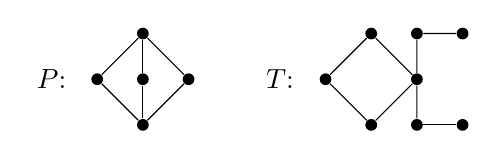
\begin{tikzpicture}[scale=0.58]%[every node/.style={circle, inner sep=0.5mm,node
                %distance=10mm,fill=black}, scale=0.2]

                \begin{scope}[xshift=-1cm, yshift=-3cm, color=black]
                \node at (-2, 1) {$P$:};
                \node [fill, circle, inner sep=1.5pt] (a) at (0,0) {};
                \node [fill, circle, inner sep=1.5pt] (b) at (-1,1) {};
                \node [fill, circle, inner sep=1.5pt] (c) at (0,1) {};
                \node [fill, circle, inner sep=1.5pt] (d) at (1,1) {};
                \node [fill, circle, inner sep=1.5pt] (e) at (0,2) {};

                \path[solid] (a) edge (b) edge (c) edge (d)
                    (e) edge (b) edge (c) edge (d);
                \end{scope}

                \begin{scope}[xshift=4cm, yshift=-3cm, color=black]
                \node at (-2, 1) {$T$:};
                \node [fill, circle, inner sep=1.5pt] (a) at (0,0) {};
                \node [fill, circle, inner sep=1.5pt] (b) at (-1,1) {};
                \node [fill, circle, inner sep=1.5pt] (c) at (1,2) {};
                \node [fill, circle, inner sep=1.5pt] (d) at (1,1) {};
                \node [fill, circle, inner sep=1.5pt] (e) at (0,2) {};
                \node [fill, circle, inner sep=1.5pt] (f) at (1,0) {};
                \node [fill, circle, inner sep=1.5pt] (g) at (2,0) {};
                \node [fill, circle, inner sep=1.5pt] (h) at (2,2) {};

                \path[solid] (a) edge (b) edge (d)
                    (e) edge (b) edge (d)
                    (d) edge (c) edge (f)
                    (c) edge (h)
                    (f) edge (g);
                \end{scope}

            \end{tikzpicture}
        \end{figure}

        \begin{figure}[t]
            \centering
            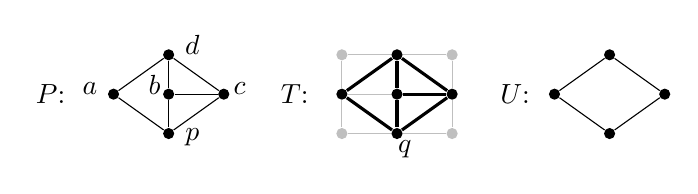
\begin{tikzpicture}[every node/.style={circle, inner sep=0.5mm}]
                \begin{scope}
                \node[fill=black] (p) {};
                \node[fill=black] (b) [above of = p,node distance=5mm] {};
                \node[fill=black] (a) [left of = b, node distance=7mm] {};
                \node[fill=black] (c) [right of = b, node distance=7mm] {};
                \node[fill=black] (d) [above of = b,node distance=5mm] {};

                \node[draw=none,right of = p,node distance=3mm,yshift=-0.5mm] {$p$};
                \node[draw=none,left of = a,node distance=3mm,anchor=base] {$a$};
                \node[draw=none,left of = b,node distance=1.8mm,anchor=base] {$b$};
                \node[draw=none,right of = c,node distance=2mm,anchor=base] {$c$};
                \node[draw=none,right of = d,node distance=3mm,anchor=base] {$d$};

                \node[draw=none, left of = a, node distance=8mm] {$P$:};

                \path (p) edge (a) edge (b) edge (c)
                    (a) edge (d)
                    (b) edge (c) edge (d)
                    (c) edge (d);

                \node[fill=gray!50] (a1) [right of = d, node distance = 2.2cm] {};
                \node[fill=black] (b1) [right of = a1, node distance=7mm] {};
                \node[fill=gray!50] (c1) [right of = b1, node distance=7mm] {};
                \node[fill=black] (a2) [below of = a1, node distance=5mm] {};
                \node[fill=black] (b2) [right of = a2, node distance=7mm] {};
                \node[fill=black] (c2) [right of = b2, node distance=7mm] {};
                \node[fill=gray!50] (a3) [below of = a2, node distance=5mm] {};
                \node[fill=black] (b3) [right of = a3, node distance=7mm] {};
                \node[fill=gray!50] (c3) [right of = b3, node distance=7mm] {};

                \node[draw=none,right of = b3,node distance=1mm, yshift=-2mm] {$q$};

                \node[draw=none, left of = a2, node distance=6mm] {$T$:};

                \path[color=gray!50] (a1) edge (b1) edge (a2)
                    (b1) edge (c1)
                    (c1) edge (c2)
                    (a2) edge (b2) edge (a3)
                    (c2) edge (c3)
                    (a3) edge (b3)
                    (b3) edge (c3);
                \path[line width=0.4mm] (b1) edge (a2) edge (b2) edge (c2)
                    (a2) edge (b3)
                    (b2) edge (c2) edge (b3)
                    (c2) edge (b3);

                \node[draw=none] (b) [right of = c2, node distance=2cm] {};
                \node[fill=black] (p) [below of = b, node distance=5mm] {};
                \node[fill=black] (a) [left of = b, node distance=7mm] {};
                \node[fill=black] (c) [right of = b, node distance=7mm] {};
                \node[fill=black] (d) [above of = b,node distance=5mm] {};

                \node[draw=none, left of = a, node distance=5mm] {$U$:};

                \path (p) edge (a) edge (c)
                    (a) edge (d)
                    (c) edge (d);
                \end{scope}
            \end{tikzpicture}
        \end{figure}
        \begin{figure}[tb]
            \centering
            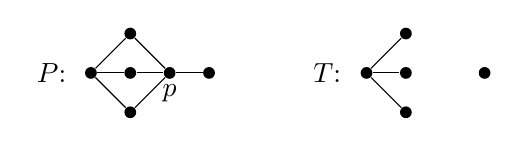
\begin{tikzpicture}[scale=0.5]%[every node/.style={circle, inner sep=0.5mm,node
                %distance=10mm,fill=black}, scale=0.2]

                \begin{scope}[xshift=-1cm, yshift=-3cm, color=black]
                \node at (-1,0) {$P$:};
                \node [fill, circle, inner sep=1.5pt] (a) at (0,0) {};
                \node [fill, circle, inner sep=1.5pt] (b) at (1,-1) {};
                \node [fill, circle, inner sep=1.5pt] (c) at (1,0) {};
                \node [fill, circle, inner sep=1.5pt] (d) at (1,1) {};
                \node [fill, circle, inner sep=1.5pt] (e) at (2,0) {};
                \node [fill, circle, inner sep=1.5pt] (f) at (3,0) {};
                \node[draw=none,below of = e,node distance=3mm,anchor=base] {$p$};

                \path[solid] (a) edge (b) edge (c) edge (d)
                    (b) edge (e)
                    (c) edge (e)
                    (d) edge (e)
                    (e) edge (f);
                \end{scope}

                \begin{scope}[xshift=6cm, yshift=-3cm, color=black]
                \node at (-1,0) {$T$:};
                \node [fill, circle, inner sep=1.5pt] (a) at (0,0) {};
                \node [fill, circle, inner sep=1.5pt] (b) at (1,-1) {};
                \node [fill, circle, inner sep=1.5pt] (c) at (1,0) {};
                \node [fill, circle, inner sep=1.5pt] (d) at (1,1) {};
                %\node [fill, circle, inner sep=1.5pt] (e) at (2,0) {};
                \node [fill, circle, inner sep=1.5pt] (f) at (3,0) {};

                \path[solid] (a) edge (b) edge (c) edge (d);
                %    (b) edge (e)
                %    (c) edge (e)
                %    (d) edge (e)
                %    (e) edge (f);
                \end{scope}

            \end{tikzpicture}
        \end{figure}
    \end{frame}




\end{document}
